\documentclass{article}
\usepackage[utf8]{inputenc}

\title{COMP280 Worksheet 3}
\author{Philip Hutchings / PH230156}

\usepackage{natbib}
\usepackage{graphicx}

\begin{document}

\maketitle

\section{Introduction}

For this assignment, I will be using a basic unity project I made which can be found using the link: (link).
It is a basic project where a cylinder game object will spawn several spheres which have a custom physics material and modified rigidbody attached to a sphere prefab. I think that it is relatively unoptimised, although it may be above a standard frames per second e.g. 60 frames per second.

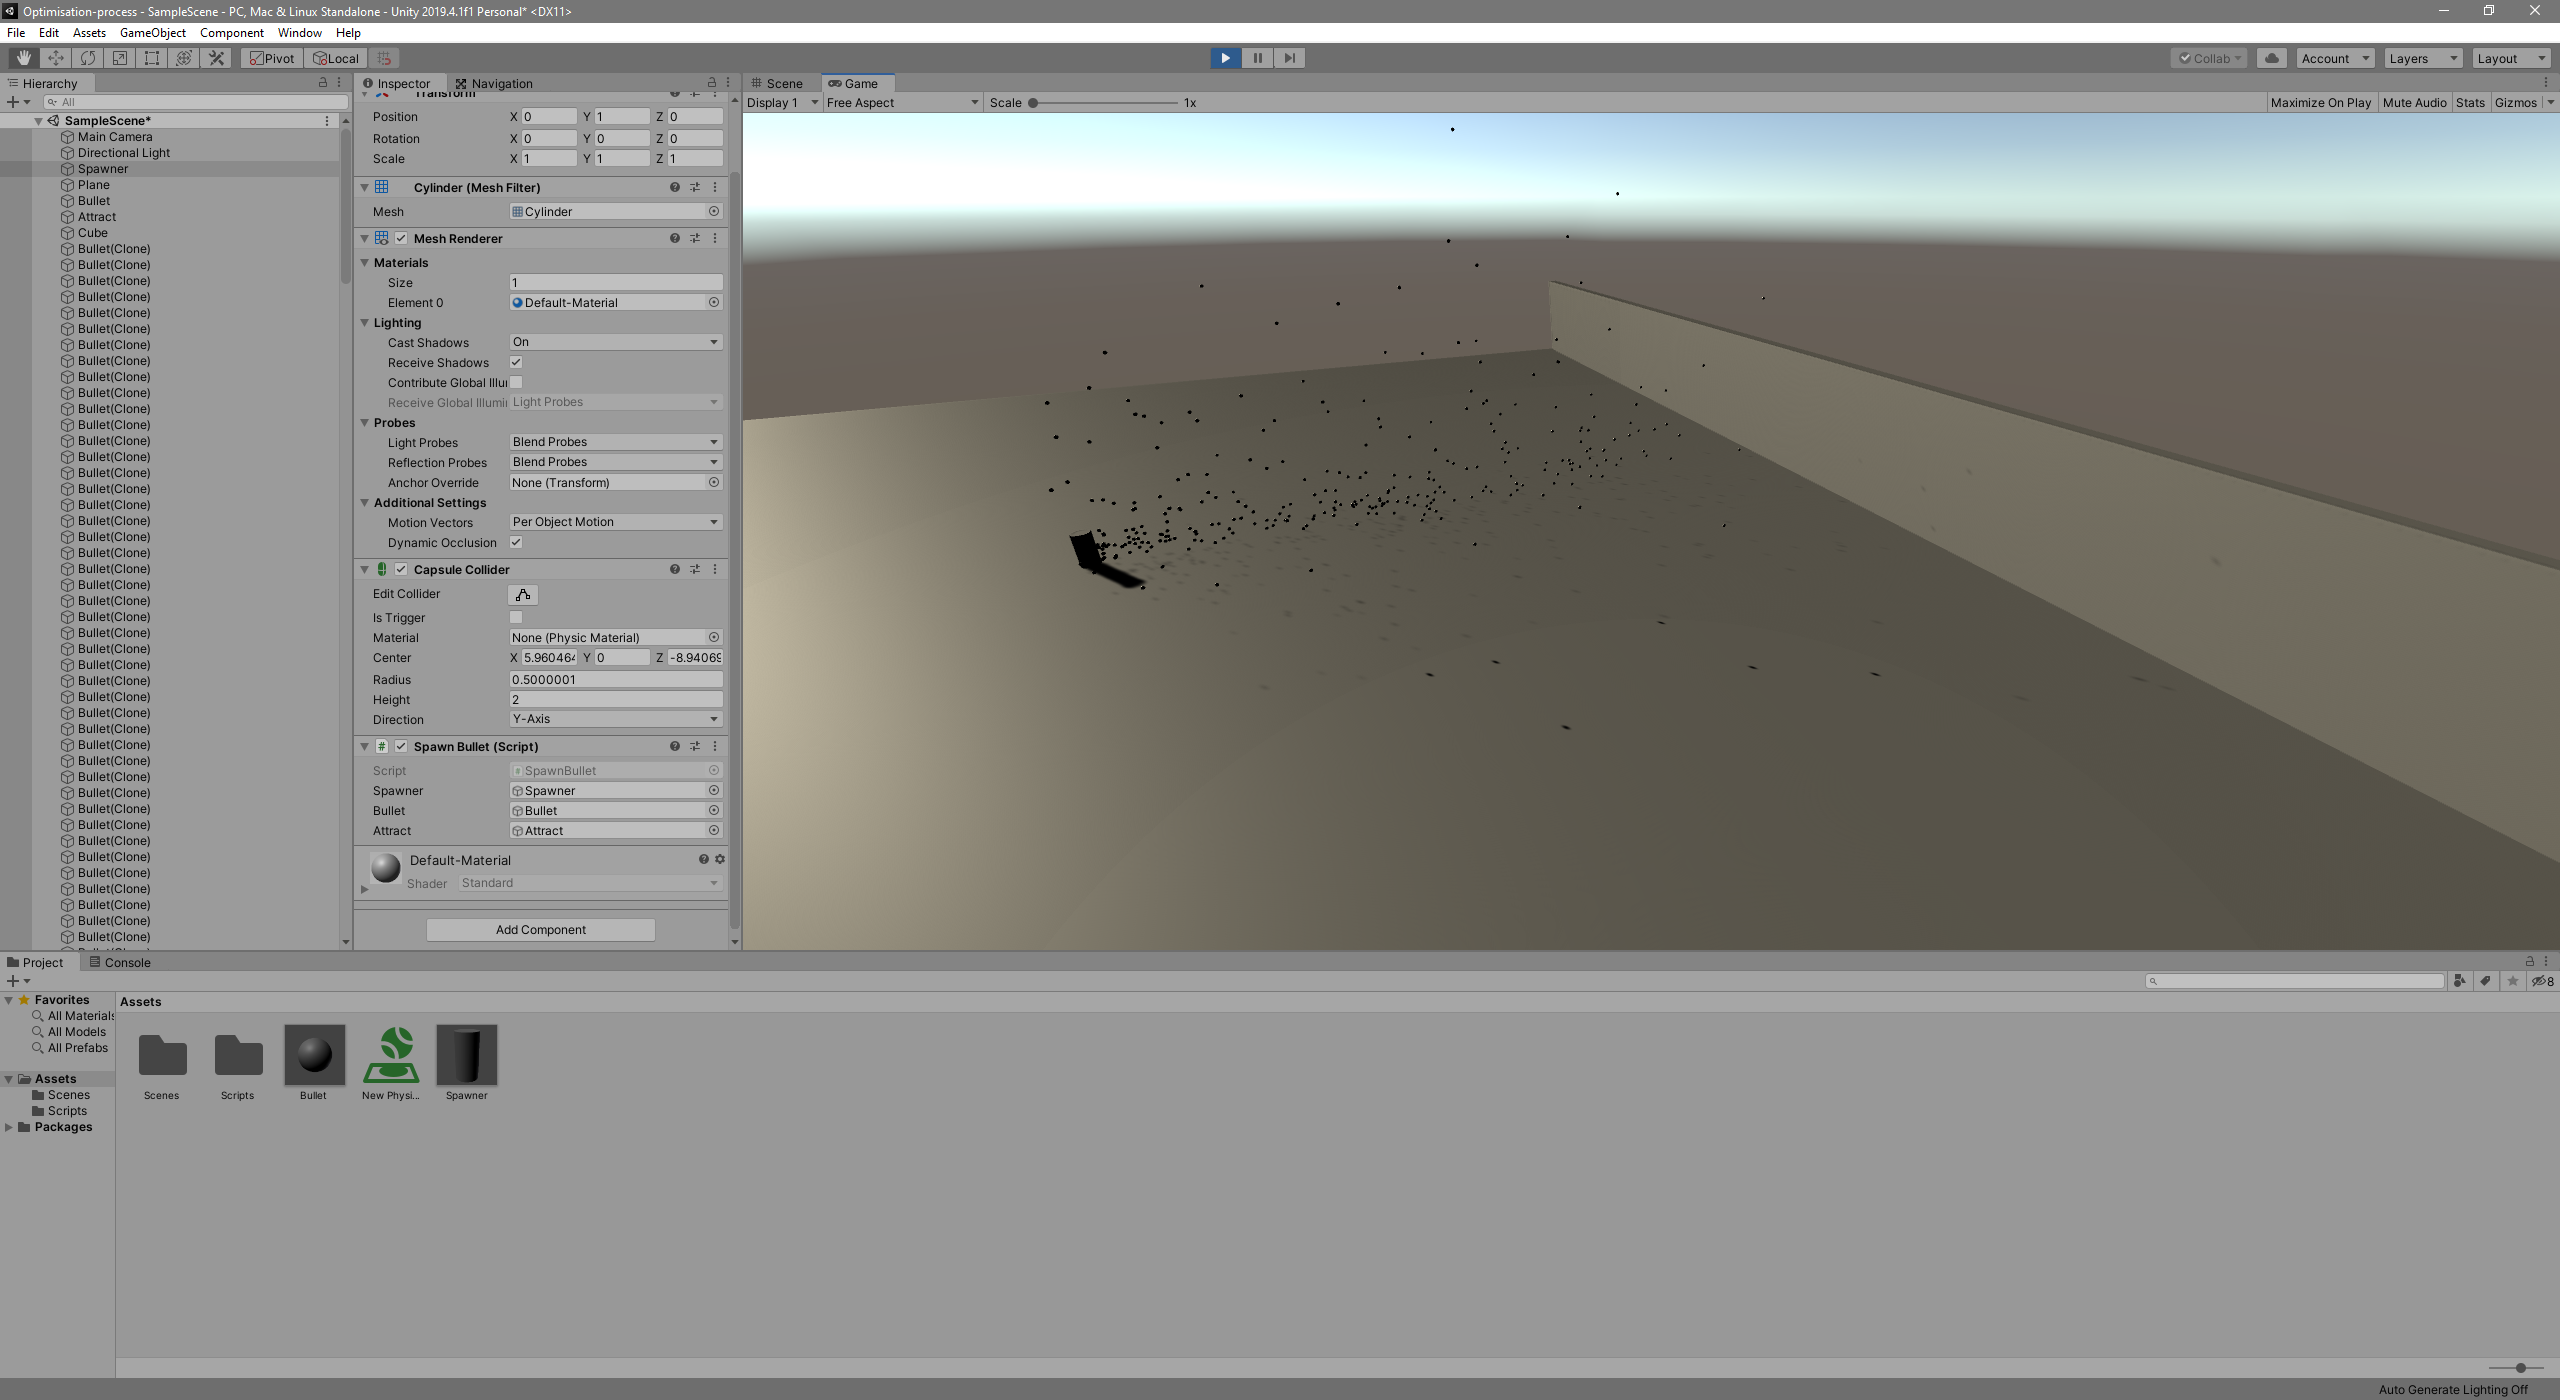
\includegraphics[width=15cm]{images/lookatproject.png}\par
A screenshot of the spheres firing out of the cylinder, though it might be hard to see.

The first thing we are doing is to look at the profiler to get an idea of how things are performing.
\section{Profiler analysis before optimisation}

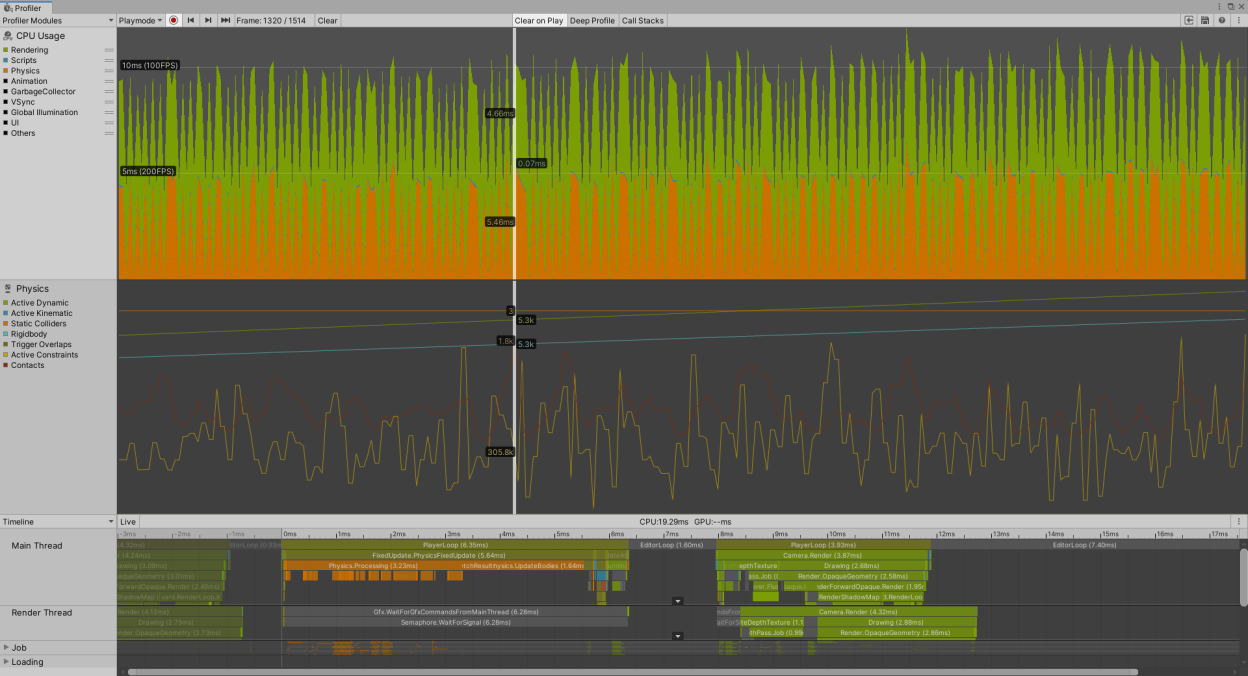
\includegraphics[width=15cm]{images/profiler.png}\par
In this screenshot, you can see the profiler window for my project. I have also turned off many of the unnecessary views such as garbage collector, vsync, etc. I have left on the rendering, scripts and physics views since these are the main contributors to my profiler statistics. 

The rendering is responsible for displaying the game to the screen, drawing objects, etc. There could be slow performance caused by objects which are being drawn when they dont need to be drawn, badly optimised code, etc.

The scripts view is responsible for showing how many resources are being used to run the scripts. The low performance could be caused by bad code or calling too many functions in one update at once.

Finally, the physics view is responsible for showing us how many constraints there are, collisions between objects, etc. The low performance from the physics could come from the sheer amount of objects with rigidbodys and physics materials, all interacting with each other at once.

\par So, first things first, we must identify the biggest contributor and optimise it in a way, in this case its physics processes.
\newpage

\section{First optimisation process}

\paragraph{} Looking at the timeline at the bottom, we can see that the main thing happening each update is a physics process.

If we take a look at my code, specifically the update function, its calling a method called "SpawnBall".

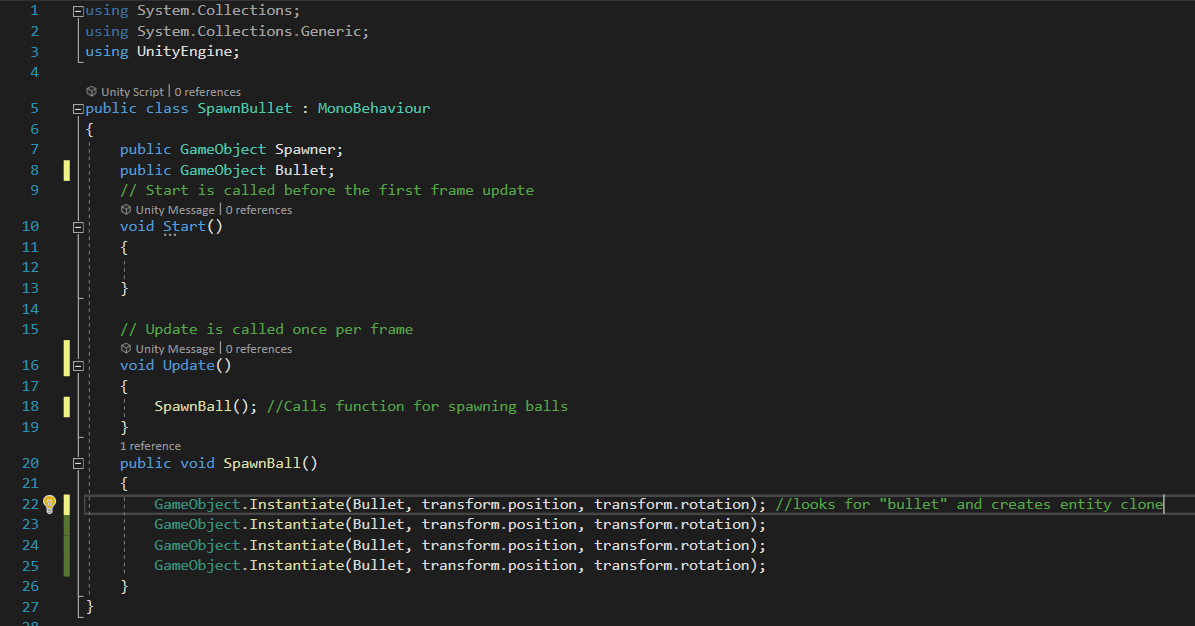
\includegraphics[width=11cm]{images/code1.png}\par
As you can see, our problem comes from the fact that it is calling the function with the intent of spawning multiple clones at once in one function call from line 22 to 25. Now I will change some code.

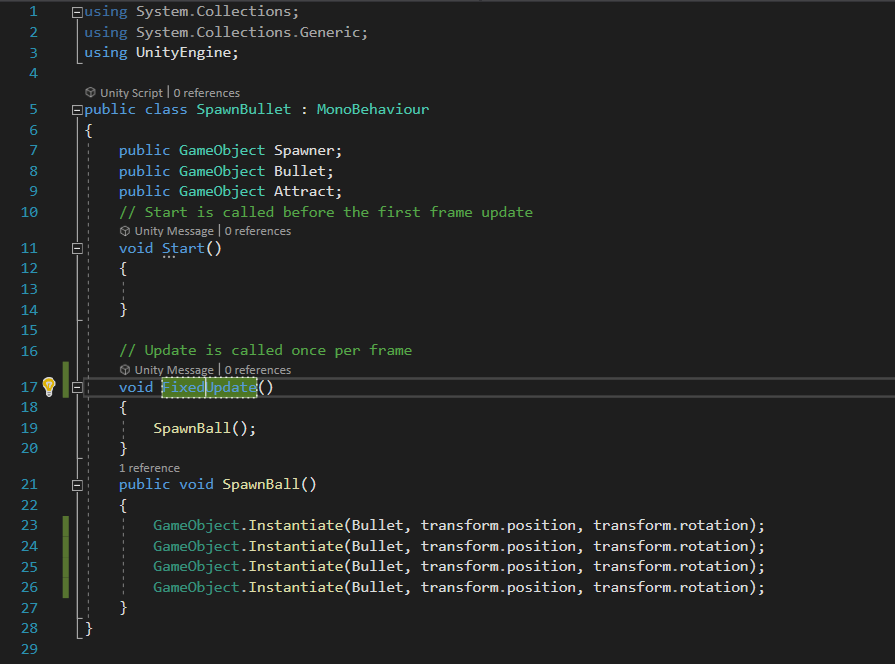
\includegraphics[width=11cm]{images/code2.png}\par
Here I have made a change to the update function, changing it from "Update" to "FixedUpdate".
\newpage

\begin{figure}
    \centering
    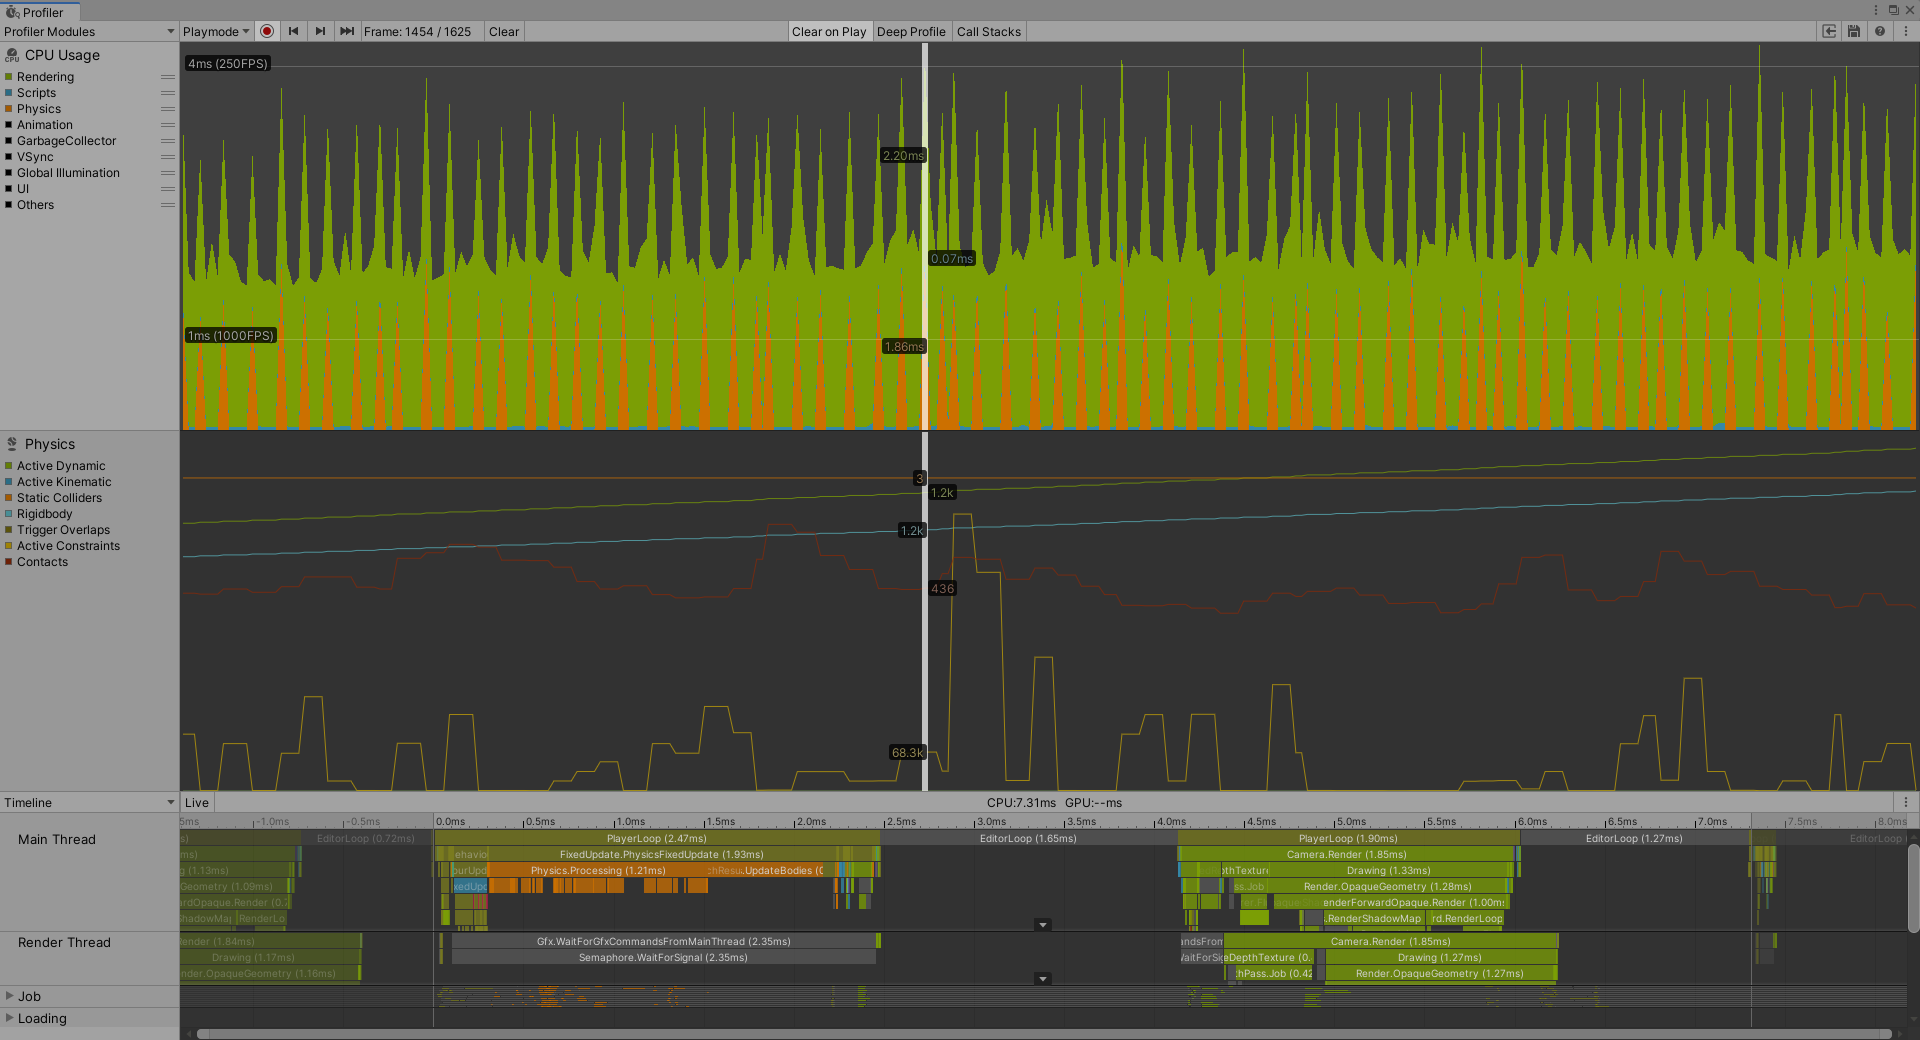
\includegraphics[width=15cm]{images/profiler1.png}
    \caption{Here is the profiler after code changes}
\end{figure}
As you can see here, we made a big difference in performance by changing the code in our script. Originally the ms on the physics processes in the CPU view were 5.46ms and after the changes it has dropped to 1.86ms. I ran the project roughly the same time to get the profiler statistics for both images(1514 frames, 1625 frames respectively). This is roughly 65 percent faster with the new code.

The next thing we will look at is the rendering processes and how we can reduce the impact on performance.
\newpage

\section{Second Optimisation process}

\paragraph{}

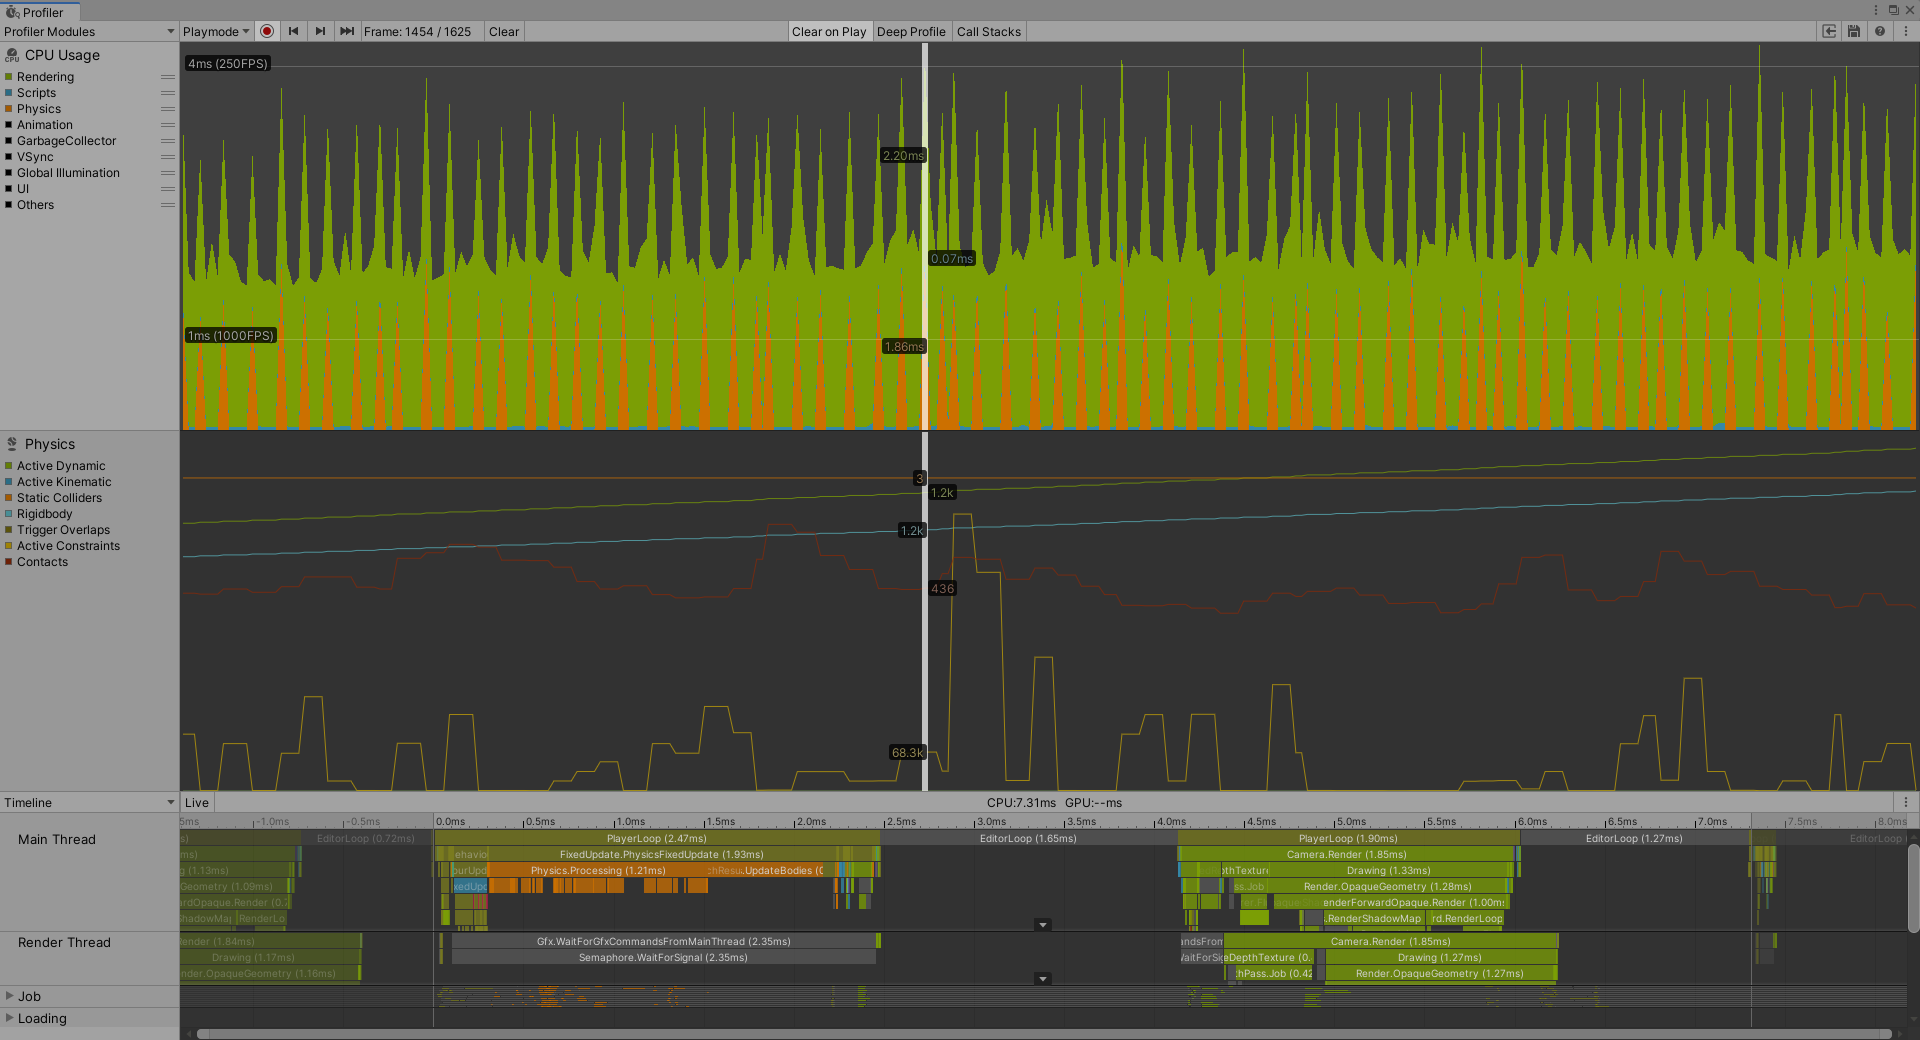
\includegraphics[width=15cm]{images/profiler1.png}
Looking at the new profiler, we can see that the rendering processes are still having a big impact on our performance, this could be happening because even if objects aren't in view, they are still being drawn. To fix this we will implement a function that removes the balls if they go below or above a certain y or x axis value. For now, the camera.render is sitting at 1.85ms in the timeline.

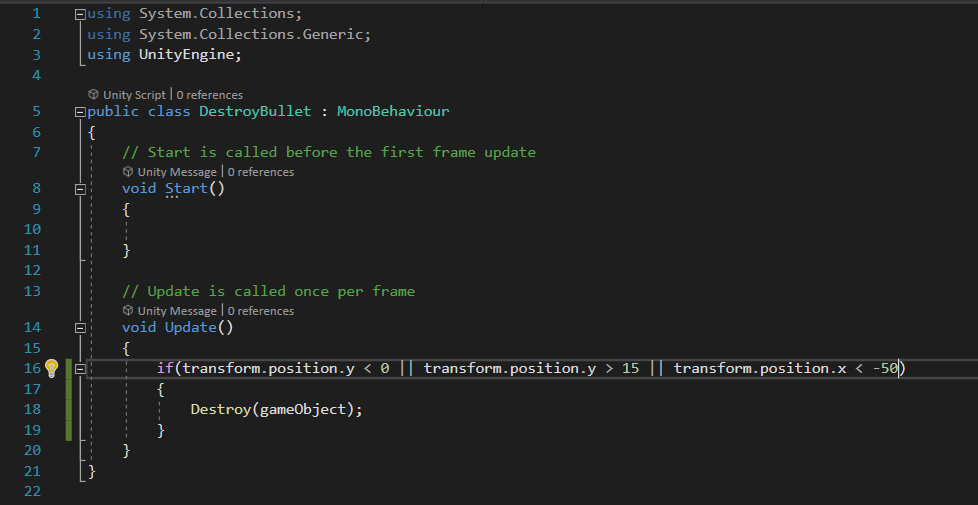
\includegraphics[width=12cm]{images/code3.png}\par
Here I have made another script to add to the ball prefab, I have made it so if a ball goes below y 0, above y 15 and beyond x -50, the object will be deleted. 
\newpage

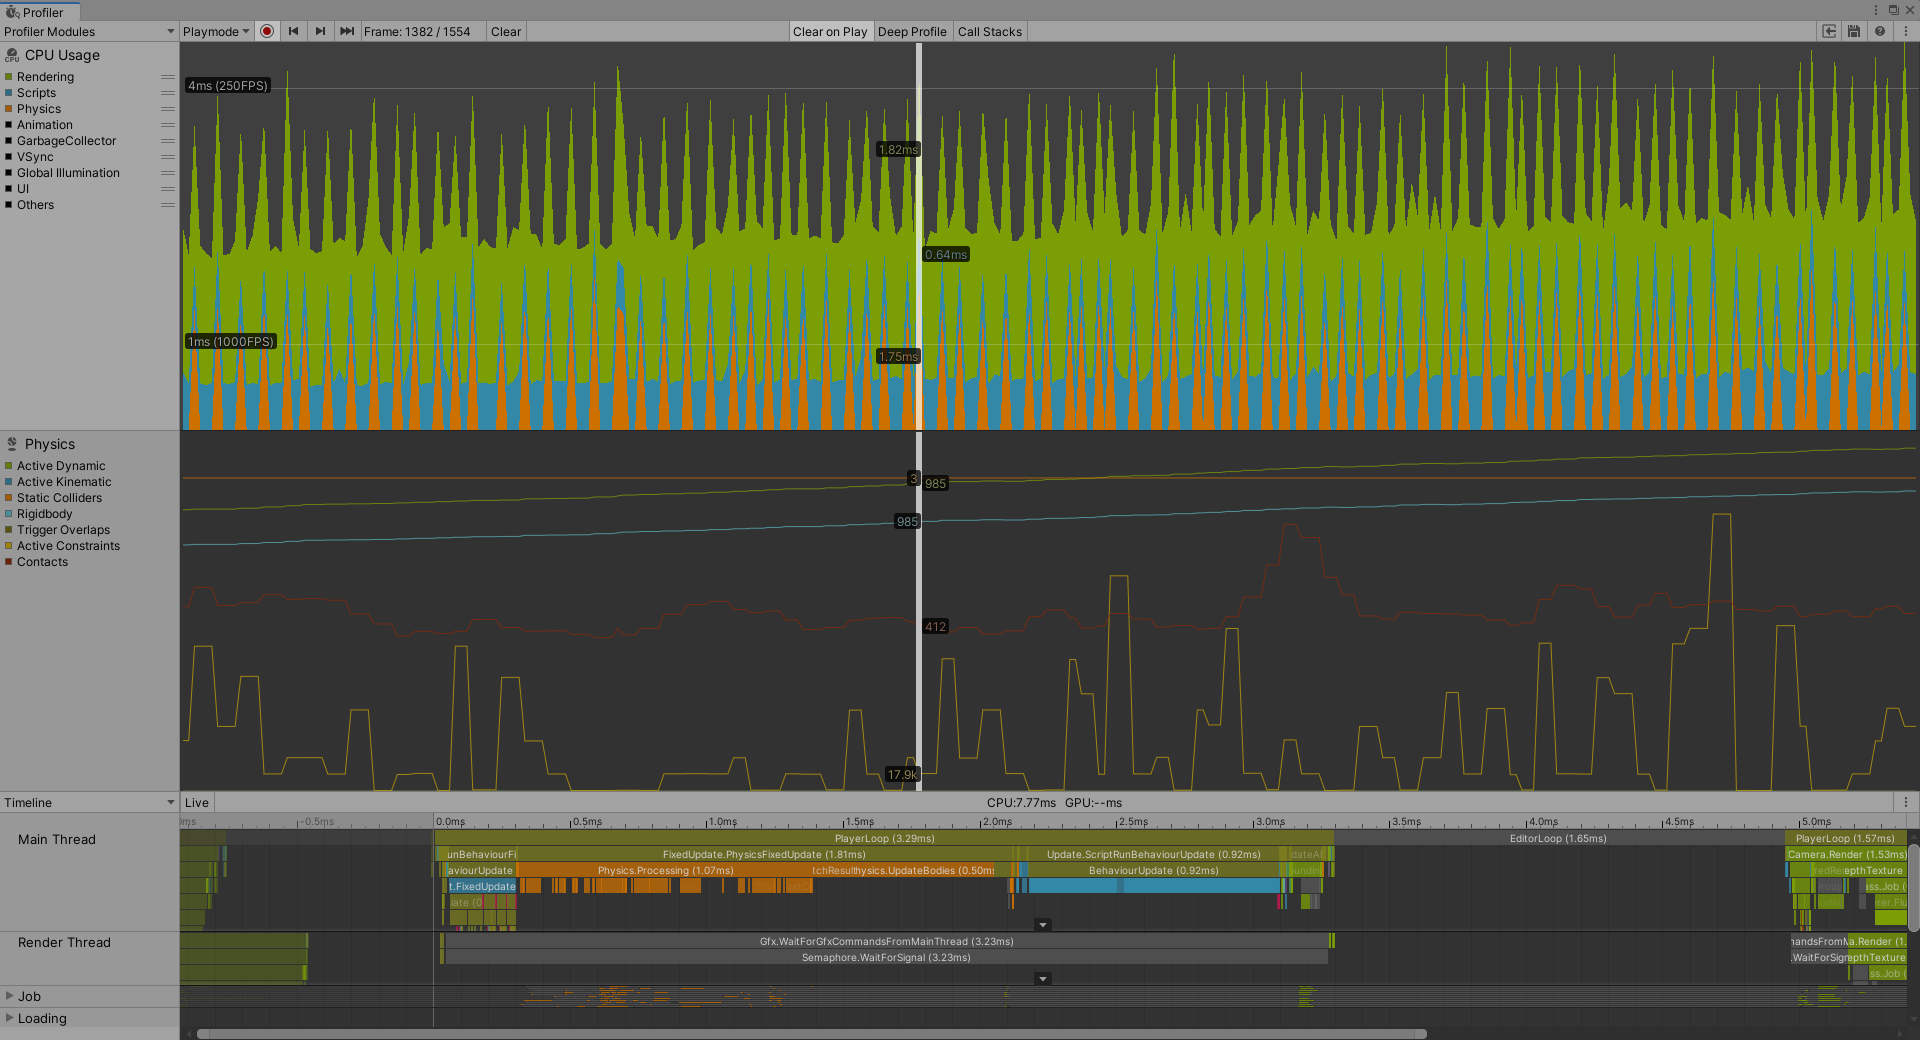
\includegraphics[width=15cm]{images/profiler3.png}\par
And as you can see in this new profiler window, the camera.render has dropped to 1.53ms(bottom right, might be hard to see), not a big difference but nonetheless it's better than before.

We can further improve the performance, not by much but in larger projects it may make a very noticeable difference.

\newpage
\section{Third optimisation process}
\paragraph{}
In this third iteration, we will make small improvements to our performance, to do this we can look in our code and remove any empty functions that we aren't using. The scripts is still taking a bit of performance away from us so we will sort that now.

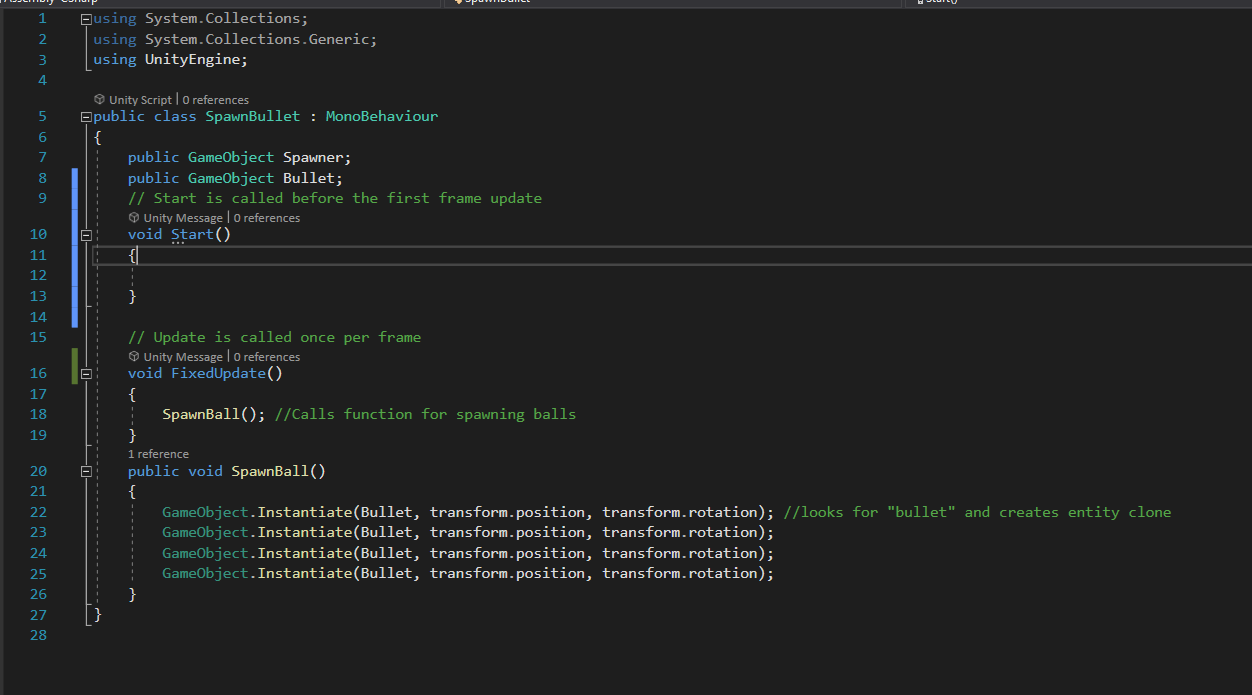
\includegraphics[width=12cm]{images/code4.png}\par
As you can see here, I have an empty function which I can remove which should hopefully lower the impact scripts is making.

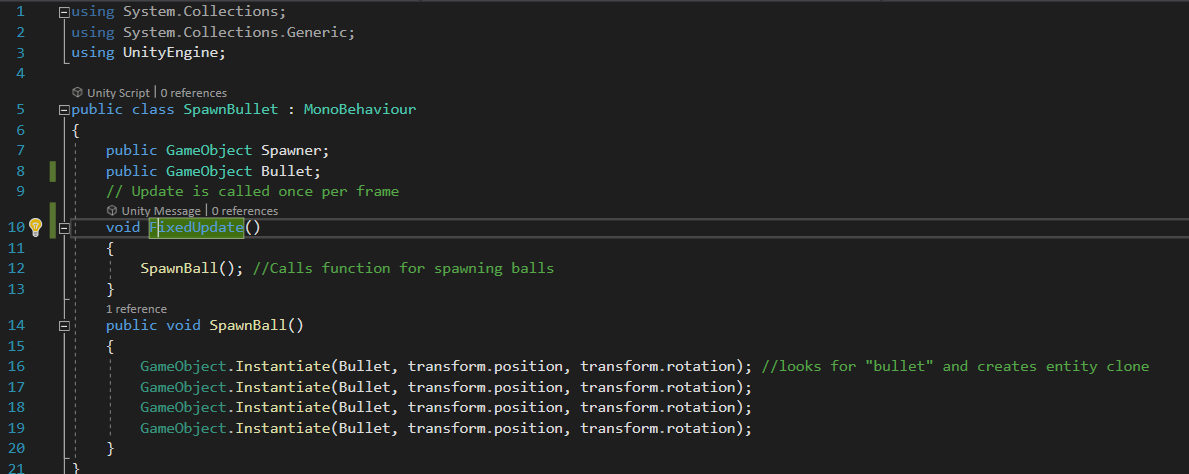
\includegraphics[width=12cm]{images/code5.png}\par
Here, you can see that I have removed the start method, now lets take a look at the profiler.

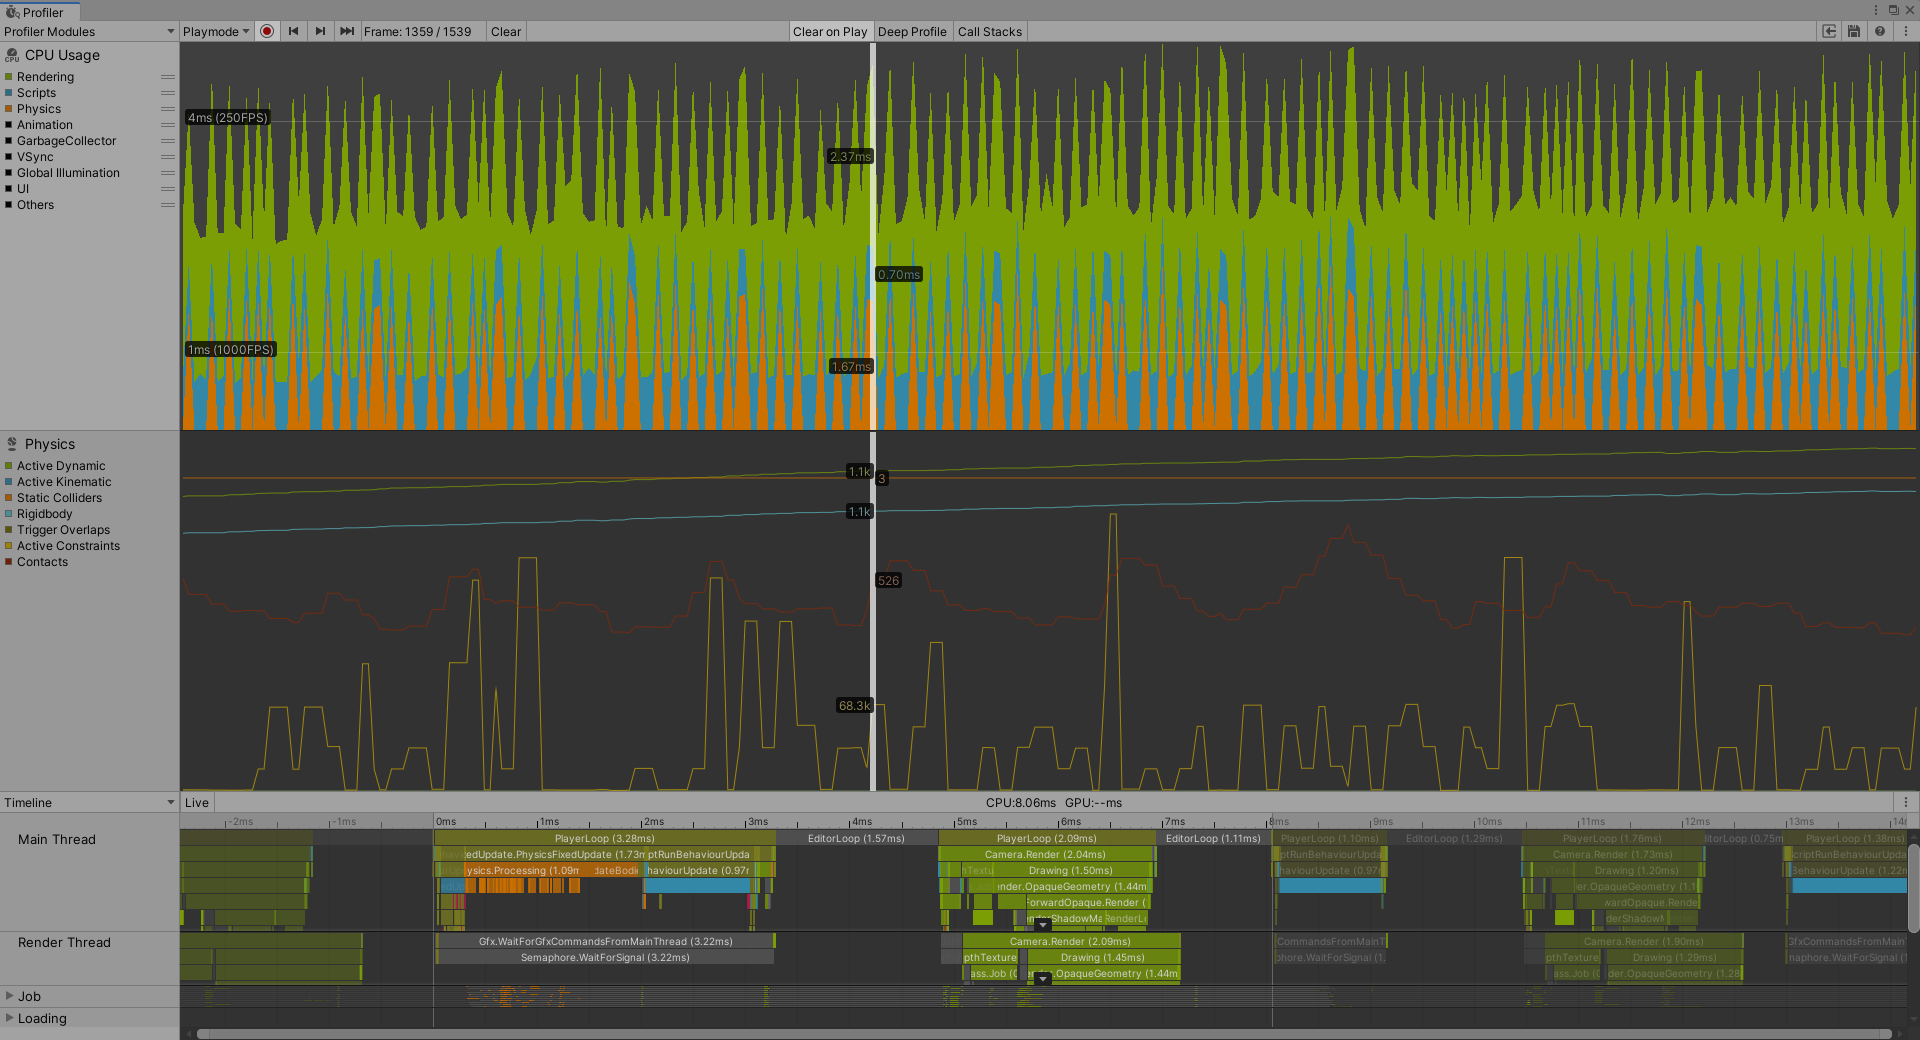
\includegraphics[width=15cm]{images/profiler4.png}\par
This here is the profiler before changes were made.

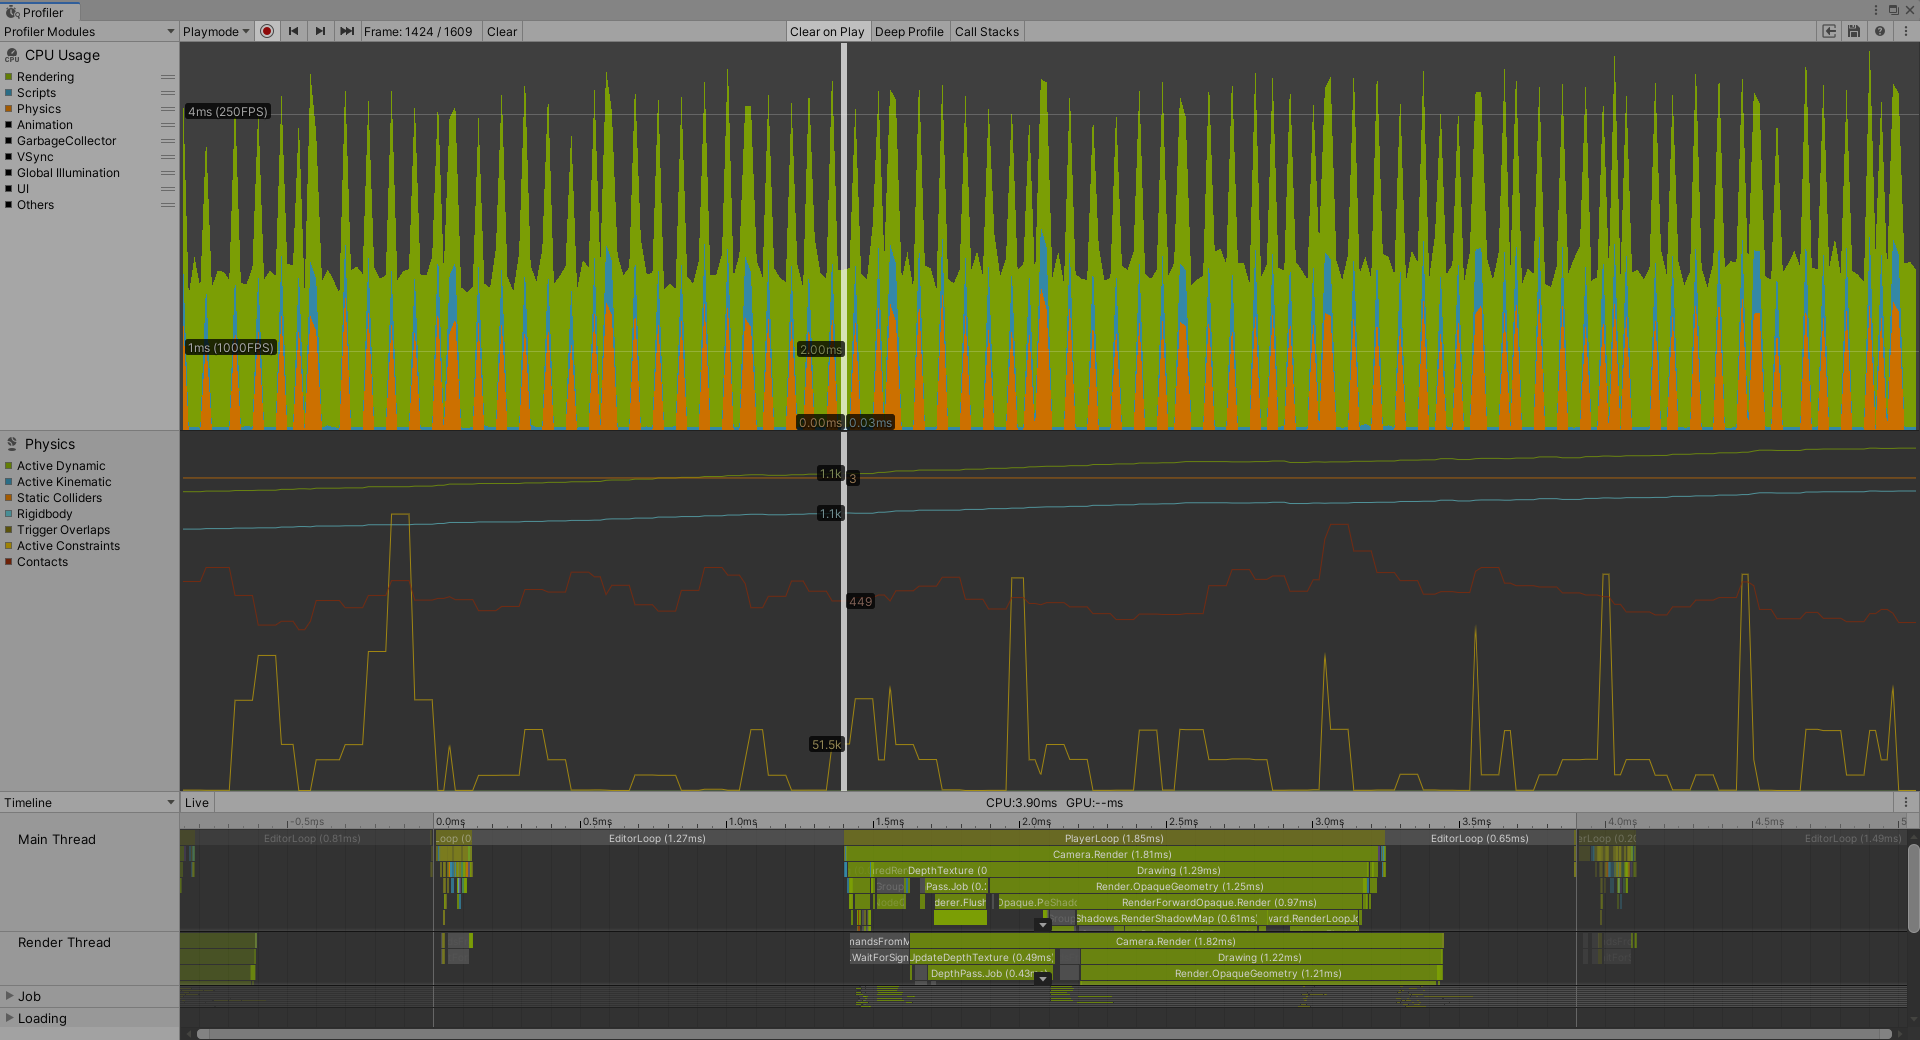
\includegraphics[width=15cm]{images/profiler5.png}\par
And this here is the profiler after the changes, and as you can see the scripts view has dropped between each update from roughly 0.70ms to about 0.03ms.
\newpage
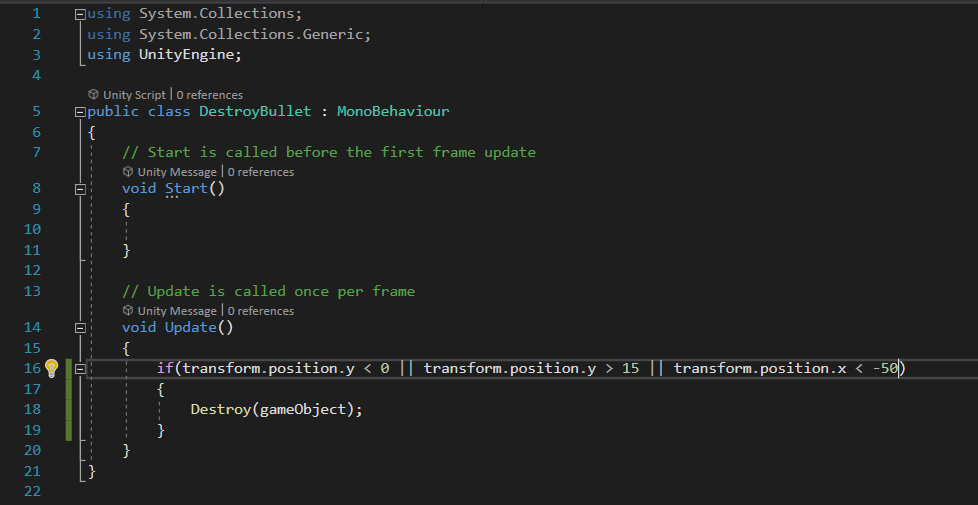
\includegraphics[width=12cm]{images/code7.png}\par
As for my other scripts "DestroyBullet", I will also do the same adjustments.

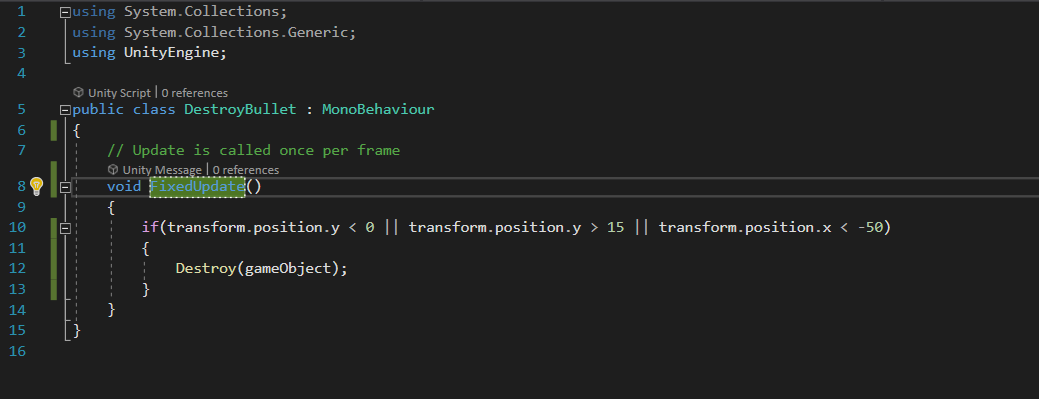
\includegraphics[width=12cm]{images/code6.png}
Here in this snippet, you can see that I have removed the start method but I have also changed "Update" to "FixedUpdate". Although these optimisations didn't have much of an impact in this project, I believe that in larger projects these optimisations will have a much bigger impact.

\end{document}
